\subsection{Concept and Approach}
\eucommentary{5-8 pages}
\eucommentary{
-- Describe and explain the overall concept underpinning the project.
Describe the main ideas, models or assumptions involved. Identify
any trans-disciplinary considerations;
-- Describe and explain the overall approach and methodology, distinguishing, as
appropriate, activities indicated in the relevant section of the work programme, e.g.
Networking Activities, Service Activities and Joint Research Activities, as detailed in
the Part E of the Specific features for Research Infrastructures of the Horizon 2020
European Research Infrastructures (including e-Infrastructures) Work Programme 2014-
2015;\\
-- Describe how the Networking Activities will foster a culture of co-operation between the
participants and other relevant stakeholders.\\
-- Describe how the Service activities will offer access to state-of-the-art infrastructures,
high quality services, and will enable users to conduct excellent research.\\
-- Describe how the Joint Research Activities will contribute to quantitative and qualitative
improvements of the services provided by the infrastructures.\\
-- As per Part E of the Work Programme, where relevant, describe how the project will
share and use existing basic operations services (e.g. authorisation and accounting
systems, service registry, etc.) with other e-infrastructure providers and justify why such
services should be (re)developed if they already exist in other e-infrastructures. Describe
how the developed services will be discoverable on-line.\\
-- Where relevant, describe how sex and/or gender analysis is taken into account in the
project's content.}

\begin{figure}
  \centerline{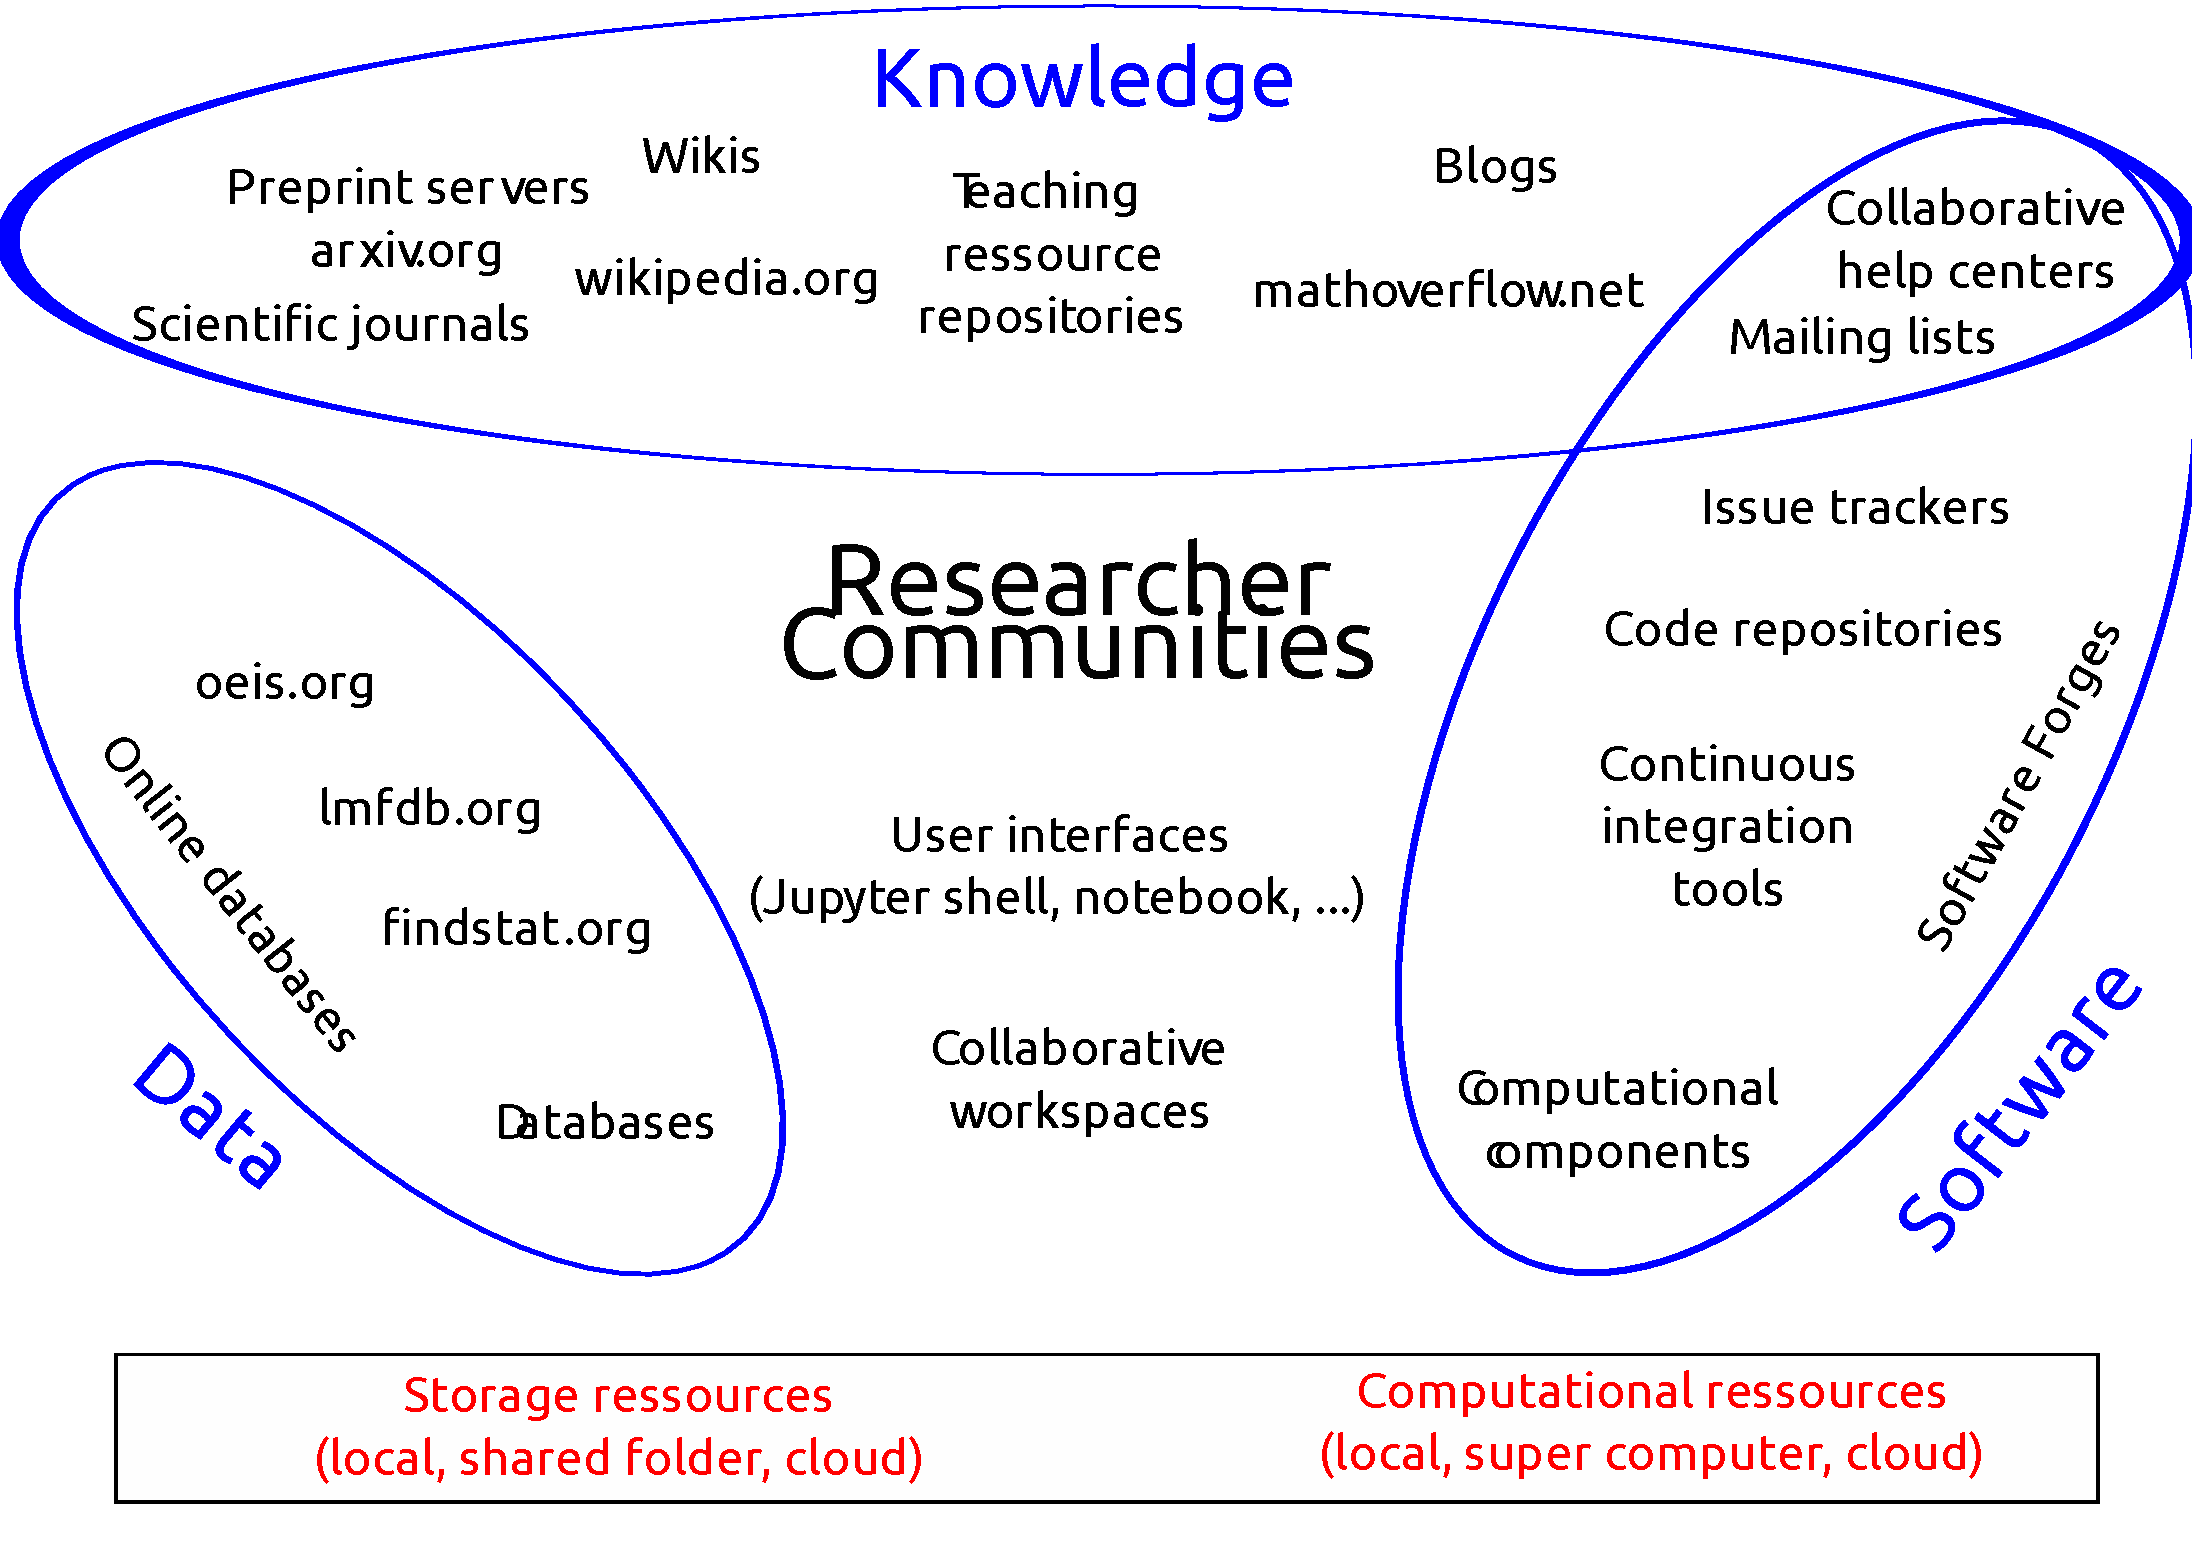
\includegraphics[width=\textwidth]{Pictures/TheBigPicture.pdf}}
  \caption{Virtual Research Environments for research in pure
    mathematics and applications.}
  \label{fig:thebigpicture}
\end{figure}

\TODO{NT: the purpose of Figure~\ref{fig:thebigpicture} is to give a quick
  sense of what Virtual Research Environments can be in our context,
  and a ``big picture'' for the project. A graphic artist friend of
  mine is going to help me improve it. I have collected here some material for her.\\\\
  \textbf{\Large What we would like the ``big picture'' in
    Figure~\ref{fig:thebigpicture} to highlight:}
  \begin{description}
  \item[This is a human centered project:] At the core: researchers and communities
    thereof.
  \item[The three types of information:]
    Software, Knowledge, Data (currently in blue)\\
    How they interact:
    \begin{itemize}
    \item Knowledge help structure data and software (e.g. through ontologies)
    \item Software produce data
    \item Data is used by researchers to build knowledge
    \end{itemize}
  \item[Physical resources:]
    (currently in red)
  \item[Virtual Research Environments]\ 
    \begin{itemize}
    \item Researchers in Math have a long tradition of collaborating
      on Software, Knowledge, and, up to some point, Data
    \item For this they use a variety of collaborative tools which
      form a loosely knit Virtual Research Environment.
    \item \textbf{Aim 2}: make it easy for subcommunities of
      researchers to setup custom collaborative work spaces / Virtual
      Research Environments tailored to their needs, by combining:
      \begin{itemize}
      \item Computational resources
      \item Storage resources
      \item Computational software components
      \item Databases
      \item User interfaces
      \item Wikis-Knowledge bases (true for findstat, LMFDB): quicker
        cycle for consolidation of information spread over
        papers/brains
      \end{itemize}
      Such VRE shall help them:
      \begin{itemize}
      \item collaboratively develop software (e.g. specialized
        libraries), data and knowledge (e.g. articles) for their
        research projects.
      \item contribute back this information to the larger community
        whenever relevant.
      \end{itemize}
    \end{itemize}
  \item[Processes:]\ \\
    It would be interesting to depict the following processes. They
    are indeed about collaboration and sharing (and quality control),
    that is what \textbf{Aim 1} is to promote.
    \begin{description}
    \item[Software development]\ 
      \begin{itemize}
      \item \emph{bug reports} and \emph{enhancement requests} emerge
        from the community, typically through collaborative help
        centers, and are posted on issue trackers.
      \item \emph{Design discussions} occur on mailing lists and issue
        trackers.
      \item Researchers \emph{submit code} to the code repositories.
      \item \emph{Quality control}: the code is reviewed and
        tested by continuous integration tools.
      \item Finally the code \emph{integrated} within computational
        components, and used by the community.
      \end{itemize}
      Researchers (as well as other users: teachers, engineers, ...)
      interact at each step of the process.
    \item[Scientific publication]\ 
      \begin{itemize}
      \item researchers submit articles to journals and post them on
        preprint servers;
      \item the articles get reviewed by other researchers;
      \item finally they are distributed back to the community
      \end{itemize}
    \end{description}
  \end{description}
  %
  Improvements to implement:
  \begin{itemize}
  \item the findstat link does not work for me, kerning looks
    extremely weird -- POD
  \item lmfdb, oeis, and findstat have a strong knowledge component as
    well, with knowls and wikis, references, ...
  \item arxiv is not far from a database of knowledge
  \end{itemize}
  %
  \textbf{\Large A collection of links that might give some idea of
    the look and feel of our universe:}
  \begin{description}
  \item[Examples of (computational) components:]\ 
    \begin{itemize}
    \item IPython: \url{http://ipython.org/}
    \item GAP: \url{http://www.gap-system.org/}
    \item Singular: \url{http://www.singular.uni-kl.de/}
    \item Sage: \url{http://sagemath.org/}
    \item \PariGP: \url{http://pari.math.u-bordeaux.fr/}
    \item Linbox: \url{http://www.linalg.org/}
    \end{itemize}
  \item[Examples of online collaborative tools]\ 
    \begin{itemize}
    \item Issue tracker: \url{http://trac.sagemath.org/timeline/}
    \item Code repository: \url{https://github.com/}
    \item Collaborative help center: \url{http://ask.sagemath.org/}
    \item Collaborative math site: \url{http://mathoverflow.net/}
    \end{itemize}
  \item[Examples of online databases]\ 
    \begin{itemize}
    \item Online databases: \url{http://oeis.org/?language=french}
    \item LMFDB: \url{http://www.lmfdb.org/EllipticCurve/Q/14.a3}
    \item Findstat: \url{http://www.findstat.org/}
    \end{itemize}
  \item[Example of graphical material]\ 
    \begin{itemize}
    \item \url{http://boxen.math.washington.edu/home/nthiery/main2014.pdf}
    \end{itemize}
  \end{description}
}

\clearpage

\subsubsection{Importance of experimental tools in pure mathematics
  and applications}

From their early days, computers have been used in pure mathematics,
either to prove theorems (e.g. the four color theorem) or, like the
telescope for astronomers, to explore new theories. By now the
experimental method, based on exact computer aided calculations, has
now been added to the standard toolbox of the pure mathematician, and
its usage has grown to the point that certain areas of mathematics now
completely depend on it.

Experiments lead to new conjectures which may have a deep impact on
the future development of mathematics. An outstanding example is the
Birch and Swinnerton-Dyer conjecture which is one of the Clay
Millenium Problems.  Databases relying on computer calculations such
as the Small Groups Library or the Modular Atlas in group and
representation theory provide indispensible tools for researchers. A
constructive way of understanding proofs of deep theorems yields
algorithmic tools to deal with highly abstract concepts. These tools
make the concepts available to a broader class of researchers, with
many potential applications. A prominent example from algebraic
geometry is the desingularization theorem of Hironaka, for which
Hironaka won the Fields Medal, and its algorithmization by Villamayor.

Spectacular theoretical breakthroughs such as the recent complete
resolution of Serre's conjectures, directly inspired by Wiles' proof
of Fermat's last theorem, are based on interdisciplinary approaches.
% Serre's conjecture was in fact proved completely within the last 10
% years, Serre is probably famous enough in Europe (?), and that work
% really is a *direct* extension of work of Wiles; at the same time, the
% conjecture of Serre and much work on it were directly inspired by big
% numerical computations (e.g., by Mestre).
Current developments on the algorithmic side allow one to conquer
crossconnections between different areas of mathematics also
computationally and, thus, to arrive at cutting-edge applications
which previously were inconceivable.

% Computational maths is interdisciplinary by nature

The field of computational mathematics allows us to compute in and
with a multitude of mathematical structures. It is interdisciplinary
in nature, with links to quite a number of areas in mathematics, with
applications in mathematics and other branches of science and
engineering, and with constantly new and often surprising
developments. Quite a number of these developments, in fact the
creation of whole subareas of the field, have been initiated by
European researchers who made crucial contributions at all
levels. These include the design of fundamental algorithms, the
development of major computer algebra systems (\TODO{this is a bit
  redundant with below}), applications of the computational methods in
various fields, and the creation of widely used databases.

Particularly fruitful interactions unfold between computer algebra and
algebraic geometry, number theory, combinatorics and group theory. Algebraic algorithms
open up new ways of accessing subareas of these key disciplines of
mathematics, and they are fundamental to practical applications of the
disciplines. Conversely, challenges arising in algebraic geometry, number
theory, combinatorics and group theory quite often lead to algorithmic breakthroughs
which, in turn, open the door for new theoretical and practical applications
of computer algebra.

\subsubsection{A long track of collaboration on software, data, knowledge}

Supporting the experimental method requires spending major efforts
on software development. As the sophistication of the required
computations increased, supported by the boom of the available
computational power, it became vital to share those efforts at the
scale of large research communities. European mathematicians have been
pioneers and have grown a steady tradition of collaborative open
source software development, with specialized systems like \GAP,
\Singular, or \PariGP playing a major role for decades.

The next scale was reached in the last decade with the advent of the
general purpose mathematical system \Sage which proved the viability
and sustainability of the ``developed by users for users'' development
model at the international level.

\TODO{This is somewhat redundant with the language in
  Objective~\ref{objective:sustainable}; see where this belongs best
  to.}

\TODO{Develop}%
Similarly, mathematicians have been building and sharing databases for
a long while; the needs for such is growing tremendously, and the
process needs to be streamlined.

\TODO{Develop}%
Mathematicians have a strong tradition of sharing knowledge openly
(arxiv, Wikipedia, ...).

% Comment by William:
% > Regarding "Mathematicians have a strong tradition of sharing knowledge
% > openly", I think one reason for this is that the landscape of math
% > research is arguably *dramatically* larger than the research landscape
% > in any other field.  As a result, mathematicians find themselves in a
% > situation where collaboration is far more rewarding and productive
% > than competition, which results in a basic culture of sharing.  In
% > sharp contrast, in areas like drug discover or physics (or perhaps
% > even more intensely, in business!), being extremely competitive and
% > secretive is frequently the best strategy.  It is thus no surprise to
% > us that mathematicians are leading the way in developing tools for
% > collaboration and sharing.      Of course, many people outside of
% > mathematics simply don't know that there is anything to mathematics
% > "beyond calculus", so they don't realize how broad our research
% > landscape is.
% > 
% > I remember a professor in chemistry or physics coming to Sage Days 7
% > at IPAM (UCLA), and remarking that he was very surprised Sage was
% > coming from "number theorists", rather than computer science (say).  I
% > would imagine that computer science is also very competitive, since
% > it's a well-funded area with many people, but compared to mathematics
% > it's basically like one relatively small research area (within
% > combinatorics...).

\subsubsection{Early VRE's}

\TODO{Motivate the relevance of VRE's, in particular by the success of
  \SMC or \Simulagora. Mention as well \LMFDB.}

\TODO{Highlight some other deployed VRE's that would benefit to the
  sorts of improvements you suggest.  You could include Wakari.io and
  also the tmpnb thing in Nature magazine:
  http://www.nature.com/news/ipython-interactive-demo-7.21492}

\subsubsection{Key concept: bringing communities together toward a VRE kit}

\TODO{Focus on VRE kit and building blocks}

\TODO{Why this focus? variability of needs, sustainability, ...}

\TODO{Bringing communities together}

\subsubsection{Linked research and innovation activities}

\eucommentary{Describe any national or international research and
  innovation activities which will be linked with the project,
  especially where the outputs from these will feed into the project;}

\TODO{For each item below, write a paragraph describing the project
  and one describing how it connects with this proposal}

\paragraph{DFG Priority Project SPP 1489}
\url{computeralgebra.de}

The SPP1489 ``Algorithmic and Experimental Methods in Algebra, Geometry, and
Number Theory'' is a nationwide Priority Project of the German Research Council DFG  
which commenced in July  2010 and will end in June 2016. The focus of the programme 
is on the interactions between computer algebra and algebraic geometry, number theory, 
and group theory. It combines expertise at all levels of research in computer algebra, 
be it the design of algorithms, the implementation of algorithms, the application
of algorithms, or the creation of mathematical databases. The goal of SPP1489 is to 
considerably further the algorithmic and experimental methods in the afore mentioned
disciplines, to combine the different methods across boundaries between the disciplines, 
and to apply them to central questions in theory and praxis. A fundamental concern of the
programme is the further development of open source
computer algebra systems with origins in Germany, which in
the framework of different projects will be crosslinked on
different levels. Of particular interest are interactions with application areas inside
and outside of mathematics such as system- and control theory, coding
theory, cryptography, CAD, algebraic combinatorics, and algebraic
statistics as well as hybrid methods which combine numerical and
symbolic approaches. 

\TOWRITE{WD}{One paragraph description of how this relates to this project}

\paragraph{IPython/Jupyter grant from the Alfred P. Sloan foundation}
\url{http://ipython.org/sloan-grant.html}

\TOWRITE{IPython}{Proofread description of the Sloan grant and link to this project}

The IPython project received a \$1.15M grant from the Alfred P. Sloan
foundation that is supporting IPython development for two years
(1/1/2013-12/31/2014), in particular at the University of California,
Berkeley and California Polytechnic State University, San Luis Obispo.
This grant enabled the project to focus on developing the IPython
Notebook as a general tool for scientific and technical computing that
is open, collaborative and reproducible. This goes a long way toward
Aim \TODO{... and ...} of \TheProject, especially given the current
rapid evolution of IPython toward its language agnostic avatar
Jupyter.

\TheProject will build on the outcome of the Sloan grant, and further
develop the critical IPython/Jupyter component in close collaboration
with the IPython/Jupyter team. In particular, we plan to hire some of
the European developers that are currently funded by the Sloan grant
to work in California and wish to later return to Europe.

\paragraph{NSF SI2-SSE OCI-1147247}

%\SageCombinat is a subproject of \Sage whose mission is "to improve
%\Sage as an extensible toolbox for computer exploration in (algebraic)
%combinatorics, and foster code sharing between researchers in this
%area".

The OCI-1147247 Collaborative Research grant ``Sage-Combinat:
Developing and Sharing Open Source Software for Algebraic
Combinatorics'' is a project funded by the National Science Foundation
from June 2012 to May 2015. The grant supports the development of
\SageCombinat, on the USA side and in areas relevant to the ongoing
research of the participants (symmetric functions, Macdonald
polynomials for arbitrary Cartan types, crystals, rigged
configurations and combinatorial R-matrices, affine Weyl groups and
Hecke algebras, cluster algebras, posets, ...), together with relevant
underlying infrastructure. The project includes three Sage Days
workshops, and cofunded one at ICERM and another in Orsay. The grant
also funds a dedicated software development and computation server for
\SageCombinat, hosted in the \Sage computation farm in
Seattle. Emphasis is placed on the development of thematic tutorials
that make the code accessible to new users. The proposal also funds
graduate student RA support, curriculum development, and other
mentoring.

The workshops and outreach actions pursued by this NSF grant have
proven to be a potent tool for connecting researchers and recruiting
\Sage users and developers. One of the role of this proposal is to
support similar community building in Europe.

This NSF grant also funded


Two of the proposers, Stein and Thiéry, are respectively PI and
foreign senior participant to this NSF grant which

This NSF grant,



 also funded some of the development of \SMC and of the
category framework in \Sage which are key assets for this proposal.


\paragraph{HPAC grant from the A.N.R.}

The french national research agency ANR has funded a 4 years project on High
Performance Algebraic Computing (HPAC) focused on the development of parallel
exact linear algebra. The consortium gathers research groups from LIP6 (Paris
6), LIRMM (Montpellier), LIP (Lyon) and LIG and LJK (Grenoble). The main goals
of the project is to first develop high performance exact linear algebra kernels
with dedicated parallel runtime, propose a domain specific language for the
parallelization of exact linear algebra libraries and their composition, invent
new algorithmic solutions for large scale parallelizations. The output of the
project is then twofolds: new computational challenges arising in algebraic
cryptanalysis will be addressed, and the open-source libraries maintained by each
group will not only integrate these advances, but will expose them in a close
integration to high level computer algebra softwares. In this process, \Sage will
start benefitting from the new shared-memory parallel code of \Linbox for the
linear algebra over a finite field.
The scope of this project is mostly focused on shared memory parallelism (except
for some challenge computations). Addressing distributed and heterogeneous
infrastructures is the next step after this project, that is be addressed in
work-package 5 of the this proposal.

\paragraph{Logilab: simulagora, cubicweb, ...}

\TOWRITE{Logilab}{One paragraph description of simulagora, cubicweb, ...}
\TOWRITE{Logilab}{How does it relate to this project}

\paragraph{\SMC} \url{https://cloud.sagemath.com/}

\TOWRITE{NT/SL/WS}{Proofread section about SMC}

% No need to specify this now that UW is part of the consortium
%This section was cowritten with William Stein, head of the \SMC project.

\SMC provides a collaborative online environment for students,
teachers and researchers to interact with \Sage and with each
other. It has \Sage and \IPython worksheets, powerful \LATEX editing
features and a full \Linux computer, all accessible from a standard
web browser. Its main design feature is to enable and promote
collaboration between groups of users. It is for example a natural
place to host a course, allowing teachers to collaborate with their
students using modern tools like \Sage and \LATEX, with facilities for
real-time communication through chat, video, and shared editing of
documents, programs and worksheets; course material can be provided as
worksheets, assignments can be distributed, collected, and returned as
well. Launched in 2013, \SMC presently hosts over 100,000 projects and
10,000 weekly active users. This fast adoption by a wide variety of
users demonstrates the relevance and the long term impact this kind of
collaborative environments can have.

Technically speaking, \SMC is a specific open-source cloud-based
Virtual Research and Teaching Environment for mathematics developed
since 2013 under the lead of William Stein, with funding from the NSF,
and Google's Education Grant program. It's currently deployed at the
University of Washington at Seattle, with a business plan in the work
for commercial support for massive on line courses, subsidizing a free
service for all other academic usage and some further \Sage
development.

In comparison \TheProject focuses on open source building blocks and
architecture to easily setup and deploy custom Virtual Research
Environments. On the one hand, \SMC will serve as prototype for
\TheProject, paving the way and showcasing important features from the
users perspective. On the other hand, basically each and every task
undertaken in \TheProject will benefit back \SMC.

\paragraph{FLINT grant?}

\paragraph{LMFDB grant}

The L-functions and Modular Forms Database (LMFDB) project originated
at a meeting at The American Institute for Mathematics (AIM) in 2007.
L-functions are ubiquitous in number theory, and have applications to
mathematical physics and cryptography. The simplest example of an
L-functions is the Riemann zeta function. Two of the seven Clay
Mathematics Million Dollar Millennium Problems deal with properties of
these functions, namely the Riemann Hypothesis and the Birch and
Swinnerton-Dyer Conjecture, that were conjectured following computational exploration.  
As well as providing a central repository
of data as a resource for researchers, through its website
\url{www.lmfdb.org}, the LMFDB provides a modern handbook, including
tables, formulas, links and references, concerning particular specific
L-functions and their sources.  Between 2008 and 2012 the LMFDB was
funded through a US National Science Foundation (NSF) Focussed
Research Grant (FRG) of around \$1M.  Since 2013, the funding of the
LMFDB has passed to Europe through a six year £2.2M Programme Grant
from the UK Engineering and Physical Sciences Research Council
(EPSRC), held at the universities of Warwick and Bristol, with
Professor John Cremona (Warwick) as its Principal Investigator (see
\url{http://www2.warwick.ac.uk/fac/sci/maths/people/staff/john_cremona/lmf}).
This grant supports six three-year postdoctoral research fellows,
mathematical researchers who work on the mathematical aspects of the
project full-time, biannual workshops, equipment and a portion of the
investigators' own time.

Almost all contributors to the LMFDB project, including those directly
supported by the EPSRC grant and the larger world-wide team of 30-50
contributors of data and code, are pure mathematicians.  Most of these
have good computational skills, but are not professional programmers
or software developers.  The LMFDB has a great need to broaden the
support it can call upon from software developers, to enhance the
project in several ways, including the computation of number-theoretic
data but more specifically in supporting the database management and
website user interface, in order to make the data more accessible and
useful to others.  The codebase of the LMFDB project is entirely open
source and hosted at github (https://github.com/LMFDB/lmfdb), written
in python with specialist modules such as flask and pymongo to manage
the website and database interface, and \Sage\ for higher-level
mathematical computations.  The LMFDB project would therefore benefit
greatly from collaboration with \TheProject as it would connect the
project with a pool of experts.  Joint workshops between the LMFDB and
\TheProject will stimulate and develop such collaboration: the LMFDB
places great importance on its workshops, which are small gatherings
of around 30 invited participants who work throughout one week on
certain specific aspects of the project, coming together in plenary
sessions to make decisions, plan and collectively approve of proposed
developments.  As a leading example of the use of databases in
mathematical research, the LMFDB will provide \TheProject\ with a real
large-scale prototype around which to develop new ideas about the
design and implementation of such databases and their associated
software.  The feasibility of such collaboration was successfully
tried at a workshop at the ICMS in Edinburgh in January 2013 on
``Online databases: from L-functions to combinatorics'', sponsored by
the NSF, AIM and the ICMS.

\paragraph{Findstat?}

\paragraph{Kwarc group}


%%% Local Variables: 
%%% mode: latex
%%% TeX-master: "proposal"
%%% End: 
